\chapter{Accelerator physics of linear colliders}
\label{LinearColliderPhysics}

\begin{chapterabstract}
Since the invention of the first particle accelerators in the late 1920s, many different forms of accelerators were invented and developed over the years. 
Even though they may differ in shape and form, they all rely on the same principles. 
After a brief introduction of these principles of accelerator physics, there will be a description of the two classes of particle accelerators that are mainly used for high-energy physics nowadays: linear and circular accelerators. 
By looking at their advantages and disadvantages, the differences between them will be highlighted.
\end{chapterabstract}
\newline

After Ernest Rutherford had demonstrated the nuclear reactions of nitrogen with alpha particles from radioactive decays in 1919, he recognized the need for other more controlled sources of accelerated particles~\cite{Rutherford}.
In the following years, physicists endeavored to develop necessary devices, and found that the key principle in particle acceleration lies in electrostatics~\cite[p. 3f]{Livingston}.

\section{Principles of particle acceleration}
\label{AccPhysics:Principles}
Charged particles are accelerated inside an electric field. 
In a time independent electric field $\vec{E}$ with potential $U$, the particle with charge $q$ experiences a change in its kinetic energy by passing through this electric field:
\begin{equation}
 \Delta E = q \int \vec{E}d\vec{r} = qU
\end{equation}
The particle's charge, expressed in the elementary charge $e$, is simply multiplied by the electric potential difference in Volts in order to calculate the gain or loss of the particle's kinetic energy. 
Out of convenience, the unit for energy in particle physics is therefore ``electronvolt'' (eV).\\
By this logic, a particle is accelerated to higher energies by applying higher and higher electrostatic fields. 
This was done in the beginning of particle accelerators by increasing the voltage applied to a capacitor and passing the charged particle through the field. 
Unfortunately, there are limits to the amount of voltage that can be applied before an electric breakdown.
The solution seems simple: putting several capacitors in a row.
But again, this can not be done with electrostatic capacitors since the field gradient between two different capacitors is directed in the opposite direction.
A particle traveling from one capacitor to the next would then lose kinetic energy again in the gap between two capacitors.
A solution was quickly found by using time dependent electric fields, which change their field  orientation periodically.\\
In simple terms, these are the key principles of linear particle accelerators.
Better accelerating structures such as drift tubes and later on superconducting radio frequency (RF) cavities were developed over the years.
The first linear accelerator using normal conducting drift tubes of increasing lengths was built and demonstrated by Rolf Wider\o e in 1928~\cite[p. 6]{Wilson}.
A schematic drawing of such a structure is shown in Figure~\ref{fig:Wideroe_Linac}.
RF fields are applied to the drift tubes such that the particles are accelerated when passing through the gaps in between the tubes.
Due to the increase in the particles' energy, the tubes need to have increasing lengths in order to guarantee the particles being accelerated by the same phase of the RF field.
\begin{figure}
\centering
\includegraphics[width=0.5\textwidth]{Figures/Wideroe_Linac.png}
\caption[Schematic layout of a Wider\o e linac]{Schematic layout of a linear accelerator with drift tubes of increasing lengths after the design by Rolf Wider\o e~\cite[p. 40]{Hinterberger}.}
\label{fig:Wideroe_Linac}
\end{figure}
\\
Nowadays, particle accelerators all over the world mainly use RF cavities instead of drift tubes.
High-power RF cavities are made of superconducting material, since its electric resistance is minimal.
Unlike before, the acceleration takes place inside the cavities, and all cavity cells are of the same length and shape.
Their characteristic shape has the effect that the electromagnetic (EM) wave inside the cavity is resonant with a high quality factor.
The quality factor $Q$ describes how large the damping of the EM wave is, as it is the ratio of the stored energy over the dissipated energy~\cite[p. 148]{Wilson}.
The larger the quality factor, the smaller the damping effect.
Figure~\ref{fig:Cavities} (a) shows a 9-cell niobium cavity developed at Deutsches Elektronen-Synchrotron (DESY) in Hamburg.
Its shape is called ``TESLA-style'', and its accelerating gradient exceeds \SI{35}{\mega\volt\per\meter} whilst it can be tuned to an RF frequency of \SI{1.3}{\giga\hertz}~\cite[p. 15f]{TDR31}.
\begin{figure}
\begin{subfigure}[b]{0.49\textwidth}
\centering
 \includegraphics[width=\textwidth]{Figures/Tesla_Cavity.jpg}
\caption[Tesla-style 9-cell cavity]{Picture of a TESLA-style 9-cell niobium cavity~\cite[p. 15]{TDR31}.}
\label{fig:Tesla_Cavity}
\end{subfigure}\hfill
\begin{subfigure}[b]{0.49\textwidth}
\centering
 \includegraphics[width=0.9\textwidth]{Figures/Cavity.png}
\caption[Electric field in a cell cavity]{Schematic drawing of the electric field lines inside a cell cavity~\cite[p. 47]{Desy_SummerStudent_Lecture}.}
\label{fig:Cavity}
\end{subfigure}
\caption[RF cavities]{The multi-cell RF cavities have a characteristic shape which is modeled in such a way that the electromagnetic (EM) RF field inside the cavities resonates. Figure (a) shows a 9-cell cavity with the ``TESLA'' shape. Figure (b) illustrates the field vectors of the EM field in the single cells of the cavity.}
\label{fig:Cavities}
\end{figure}
The RF field direction inside a cell is oscillating with the RF frequency, and neighboring cavity cells show opposite field directions (see Figure~\ref{fig:Cavities} (b)).
The frequency is then tuned such that the beam always experiences an accelerating RF phase.
In comparison to the drift tubes explained above, the matching of the particles to the wanted accelerating RF phase is therefore done here by time dependent frequencies, whilst for the drift tube structures it is done purely by the change in the geometry of the tubes.
\\
The development of the linear accelerating structures remains a significant factor for modern particle accelerators.
Nevertheless, also the advance in the research efforts for other accelerator designs has an essential impact:
The drift tube linac (short for linear accelerator) was not the only accelerator concept developed by Rolf Wider\o e, he even more importantly invented the very first accelerating structures using magnetic fields.
By using a magnetic field, the charged particles are deflected on a radial path, which therefore allows the accelerator to be much smaller than before~\cite[cf. p. 8]{Wilson}.
This idea was needed in order to advance from purely linear to circular particle accelerators.


\section{Transverse beam dynamics}
\label{AccPhysics:Magnets}

Although completely new accelerator designs are now possible by using magnetic fields, circular acceleration of charged particles has certain challenges.
From the equilibrium of the Lorentz and the centripetal force follows:
\begin{align}
q(\vec{v}\times \vec{B}) &= \frac{m\vec{v}^2}{\vec{r}}\\
qvB\vec{e_r} &= \frac{mv^2}{r}\vec{e_r} \nonumber \\
 r&=\frac{mv}{qB}\\
 &=\frac{p}{qB}\label{eq:MagField_Radius}
\end{align}
Since the momentum $p$ of the charged particle rises over time during the acceleration, the radius $r$ of its circular path increases if the magnetic field $B$ is constant.
The accelerator hence has to be built accordingly, taking the increase in the radius into account, or needs to use magnets with variable field strengths.
The latter is done in synchrotron machines, a type of circular accelerator combining the principles of all particle accelerators mentioned above: acceleration in RF cavities, variation of the RF frequency, and variable magnetic field strengths.
In this way, the particles are traveling along a stationary orbit, passing through the same bending dipole magnets and cavities over and over again until the desired beam energy is reached.\\
To insure the stability of the orbit, additional quadrupole magnets focus the beam horizontally and vertically onto the ideal particle orbit.
However, as the focal length of these quadrupole magnets depends on the particle momentum, off-momentum particles due to the natural spread in the particle energy cause the quadrupoles to introduce so-called chromatic aberrations.
Therefore, also sextupole and possibly octupole magnets are needed, which then correct orbital fluctuations.
The need for higher order correction magnets can also be derived from the expansion of the magnetic field around the ideal path of the particle (x = 0):
\begin{alignat}{5}
 B_y(x) &= B_{y0} &&+ \frac{\partial B_y}{\partial x}x &&+ \frac{1}{2!}\frac{\partial^2 B_y}{\partial x^2}x^2 &&+ \frac{1}{3!}\frac{\partial^3 B_y}{\partial x^3}x^3 &+ ...\\
 \intertext{When multiplying with $\frac{q}{p}$:}
 \frac{q}{p}B_y(x) &= \frac{q}{p}B_{y0} &&+ \frac{q}{p}\frac{\partial B_y}{\partial x}x &&+  \frac{1}{2!}\frac{q}{p}\frac{\partial^2 B_y}{\partial x^2}x^2 &&+ \frac{1}{3!}\frac{q}{p}\frac{\partial^3 B_y}{\partial x^3}x^3 &+ ...\\
  &= \frac{1}{r} &&+ kx &&+ \frac{1}{2!}mx^2 &&+ \frac{1}{3!}ox^3 &+ ... \label{eq:field_components}\\
  &\rightarrow \textnormal{dipole} &&+ \textnormal{quadrupole} &&+ \textnormal{sextupole} &&+ \textnormal{octupole} &+ ...\nonumber
\end{alignat}
and equivalently from $B_x(y)$.
\\Equation~\ref{eq:field_components} shows the connection between the radius and the magnetic field in the dipole component (using Equation~\ref{eq:MagField_Radius}).
In the quadrupole, sextupole and octupole components, factors for the magnet strength are introduced.
According to the Maxwell equation $\vec{\nabla}\cdot\vec{B} = \frac{\partial B_y}{\partial x} -\frac{\partial B_x}{\partial y} = 0$, the Lorentz force on a particle in a quadrupole magnet, has therefore to be written as (cf. \cite[p. 372]{VacuumElectronics}):
\begin{multicols}{2}
\noindent 
\begin{align}
 F_x &= -qv\frac{\partial B_y}{\partial x}x \nonumber\\
  &= -q\beta c\frac{\partial B_y}{\partial x}x\\
  &= -gx\label{eq:Quad_Lorentz_x}
\end{align}
\columnbreak
\begin{align}
 F_y &= qv\frac{\partial B_x}{\partial y}y\nonumber \\
  &= q\beta c\frac{\partial B_x}{\partial y}y\\
  &= gy \label{eq:Quad_Lorentz_y}
\end{align}
\end{multicols}
From the opposite signs in Equations~\ref{eq:Quad_Lorentz_x} and \ref{eq:Quad_Lorentz_y}, it becomes clear that quadrupoles can only focus in one direction, whilst they defocus in the other.
A schematic cross section of a quadrupole magnet is shown in Figure~\ref{fig:Quadrupole}, in which a positively charged particle beam would be focused in the y-direction and defocused in the x-direction. 
The magnetic field lines point from the magnetic north pole to the south pole, and get denser towards the edges of the beam pipe.
The further a beam particle is away from the center, the stronger is the magnetic field it experiences, and the more it is deflected towards (or away from) the center, much like light in an optical lens.
\begin{figure}
\begin{subfigure}[t]{0.49\textwidth}
\centering
 \includegraphics[width=0.9\textwidth]{Figures/Quadrupole.png}
\caption[Cross-section of a quadrupole magnet]{Schematic cross section of a quadrupole magnet with the four magnetic north and south poles.
The beam pipe is centered in the middle between the pole shoes~\cite[p. 88]{Hinterberger}.}
\label{fig:Quadrupole:cross_section}
\end{subfigure}\hfill
\begin{subfigure}[t]{0.49\textwidth}
\centering
 \includegraphics[width=0.9\textwidth]{Figures/Magnetic_field_quadrupole.png}
\caption[Magnetic field in an ideal quadrupole magnet]{Magnetic field lines inside an ideal quadrupole magnet~\cite{QuadrupoleField}.
The field lines are directed from the north to the south poles, and become denser towards the edges.
At any given point, the direction of the magnetic field (B) and the resulting Lorentz force (F) can be determined.
A beam of positively charged particles going into the page would be focused in the y-direction and defocused in x.}
\label{fig:Quadrupole:field_lines}
\end{subfigure}
\caption[Schematic drawings of a quadrupole magnet]{Schematic drawings of the cross section of an ideal quadrupole magnet (a), and of the magnetic field lines in the center of such a quadrupole magnet (b).}
\label{fig:Quadrupole}
\end{figure}
\\
Due to the fact that there are focusing and defocusing quadrupoles, so-called FODO structures are commonly used in particle accelerators.
FODO is an alternating structure made out of focusing quadrupole magnets (``F'') and defocusing ones (``D''), with drift paths (``O'') in between (see Figure~\ref{fig:FODO}). 
The naming only refers to one of the planes (either horizontally or vertically), since a quadrupole focuses horizontally whilst it defocuses vertically or vice versa.
Theoretically, a ``FODO'' cell in x is therefore a ``DOFO'' cell in y.
Hence, several of these structures, which act like optical lenses, are needed to focus the particle beam in both directions, horizontally and vertically.
\begin{figure}
\centering
\includegraphics[width=0.5\textwidth]{Figures/FODO.png}
\caption[Schematic of FODO structure]{Schematics of a FODO structure in the horizontal and vertical plane. The particles are focused and defocused by the quadrupoles that act as lenses~\cite[p. 65]{Hinterberger}.}
\label{fig:FODO}
\end{figure}
Due to the restoring force, particles that were deflected by the focusing magnets start to perform betatron oscillations around the ideal particle trajectory.
The amplitude of these oscillations is the beam envelope that covers the paths of all beam particles, i.e. the transverse beam dimension at a given location.
It can be expressed by the two beam parameters $\beta$ and $\epsilon$ which will be explained in the following:
\begin{itemize}
 \item The beta function $\beta$ describes the spatial dependency of the amplitude and the wave length of the betatron oscillations.
It is a periodic function, dependent on the focusing strengths and the location of the magnets along the beam path.
At any given point along the path, the $\beta$ value can be given in units of length.
Of particular interest is its value at the interaction point (IP), the point of the beam collisions, where it is then called $\beta^*$.
In order to minimize the beam size at the IP, the beta function is tailored such that it has a local minimum at this point.  
\item Like the beta function, the transverse emittance $\epsilon$ is defined in the horizontal and vertical plane.
In simple terms, $\epsilon$ is a direct measure of the convergence of the beam with respect to its spread in space and in transverse momentum.
A small emittance therefore means that the beam particles are confined to a small space, with a narrow transverse momentum distribution.
It also has the units of length, and is often given as the normalized emittance $\epsilon^* = \epsilon\beta\gamma$, with $\beta=\frac{v}{c}$ the relativistic Lorentz factor $\gamma=\frac{1}{\sqrt{1-\beta^2}}$.
\end{itemize}
Together, the spatial amplitude of the betatron oscillations can be written as $\sqrt{\epsilon\beta}$.
Since the amplitude of these oscillations counts towards the size of the beam, its contribution to the beam size can then be written as $\sigma_{betatron} = \sqrt{\epsilon\beta}$.
The amplitude is also shown as the maximum extent in x in the so-called phase-space ellipse, shown in Figure~\ref{fig:PhaseSpaceEllipse}.
The phase-space is spanned by x and x', where x can stand for the x and y-direction). 
x represents the position of the particle, and x' represents the change in position along the particle trajectory $s$, so that x'$=\frac{d\rm{x}}{ds}$.
The beam emittance $\epsilon$ can be defined in terms of the phase-space ellipse more accurately than it was done above.
$\epsilon$ is hence defined as the area (divided by $\pi$) of the phase-space ellipse.\\
The ellipse drawn in the phase-space illustrates the qualities of the particle beam.
Since the particles' spread in position and momentum varies along the beam line, the shape of the ellipse changes constantly, but the area of the ellipse stays the same for energy-conserving systems.
The normalized emittance $\epsilon^*$, which was explained above, is the quantity which is adiabatically invariant under energy change.
\begin{figure}[h]
\centering
\includegraphics[width=0.5\textwidth]{Figures/PhaseSpaceEllipse_w_AxisTitles.png}
\caption[Phase space ellipse]{Phase space ellipse~\cite[based on p. 158]{Wiedemann}
\\The variables $\alpha$ and $\gamma$ are defined here as: $\alpha = -\frac12\beta'$ and $\gamma = \frac{1+\alpha^2}{\beta}$~\cite[cf. p. 283ff]{Wangler}.}
\label{fig:PhaseSpaceEllipse}
\end{figure}
\\
The actual transverse size of the beam is not yet fully defined by the spatial amplitude of the betatron oscillations~\cite[cf. p. 108ff]{Conte}.
The deviation from the ideal particle trajectory due to the momentum spread has to be taken into account, which is defined by the dispersion function $\eta$.
Like $\epsilon$ and $\beta$, it is dependent on the position along the beam trajectory, and can be defined as $\eta = \frac{dx}{d\delta}$, with the fractional deviation from the ideal particle momentum $p_0$: $\delta = \Delta p/p_0$.
\\
With this knowledge, the overall beam size can be calculated by using the betatron oscillation amplitude as well as the spread in the particle momentum distribution for all particles:
\begin{align}
 \sigma&=\sqrt{\sigma^2_{betatron}+\sigma^2_{dispersion}}\\
 &=\sqrt{\epsilon\cdot\beta+\left(\eta\frac{\Delta p}{p_0}\right)^2}
\end{align}

\section{Longitudinal beam dynamics}
\label{AccPhysics:Bunching}

Apart from the transverse beam dynamics, there are also effects in the longitudinal direction, concerning the movement of the particles along the beam trajectory.
As mentioned above, both modern accelerator concepts, linear accelerators as well as synchrotrons, use  RF cavities in order to accelerate the particles.
Due to the nature of these accelerating structures, there is a certain phase of the RF frequency that can accelerate the particles in an optimal way.
In order to provide this ideal acceleration to all beam particles, the beam has to be bunched.\\
In circular accelerators, this bunching happens naturally due to the choice of the RF frequency and the timing of the beam arriving at the accelerating cavities.
The RF frequency is chosen such that the particles with the ideal momentum $p_0$ arrive at the cavity at the synchronous phase $\psi_s$, which is off the crest of the RF wave.
Depending on the system,  $\psi_s$ is then appointed to be either on the rising or the falling edge of the accelerating RF wave, or at the zero crossing.
In a circular accelerator, such as a storage ring, the particles are to be constantly accelerated and longitudinally focused at the same time.
$\psi_s$ is therefore off-crest on the falling edge of the RF wave.
For relativistic particles traveling at the speed of light, their orbit along the storage ring depends on the difference of their momentum $\Delta p$ to the ideal momentum $p_0$.
Particles with a smaller momentum travel on an orbit that is smaller than the ideal orbit.
This is due to the fact that the radius of the particle's path in a magnetic dipole field depends on the momentum of the particle, which is shown in Equation~\ref{eq:MagField_Radius}.
These particles on a smaller orbit will arrive at the next accelerating cavity earlier than the ideal particles (which arrive at the synchronous phase $\psi_s$), and will therefore experience a larger field which accelerates the particles to higher energies.
Particles that have energies larger than the ideal particles are deflected onto a larger orbit and will therefore arrive late at the RF cavity, where they then gain less energy. 
Hence, particles are accelerated by different phases of the RF field, as can be seen in Figure~\ref{fig:RFPhase}.
Particles arriving later will be accelerated less, particles arriving too early will be accelerated more.
The particles oscillate about this ideal stable phase $\psi_s$, and are therefore focused longitudinally.
This effect is called ``phase focusing''.
\begin{figure}
\begin{subfigure}[b]{0.4\textwidth}
\centering
 \includegraphics[width=0.9\textwidth]{Figures/PhaseFocusing.png}
\end{subfigure}\hfill
\begin{subfigure}[b]{0.49\textwidth}
\centering
 \includegraphics[width=0.9\textwidth]{Figures/RFphase.png}
\end{subfigure}
\caption[Phase focusing]{Relativistic charged particles with the ideal momentum ($\Delta p/p = 0$) travel on the ideal orbit of the accelerator, and arrive at the next accelerating RF structure at the RF phase $\psi_s$, the so-called ``synchronous phase''. 
Particles with a smaller momentum ($\Delta p/p < 0$) travel on a shorter orbit, and will arrive earlier than the ideal particles.
These particles will therefore be accelerated more, whilst particles with larger momentum will be accelerated less respectively.
Illustrations based on~\cite{Anke}.}
\label{fig:RFPhase}
\end{figure}

However, in linear accelerators bunching is done differently and in several stages.
The initial bunching is done directly after the particle source, which is the very first stage of acceleration.
As the particles at this stage are still non-relativistic, one of the possible methods that can be used is ``velocity bunching''~\cite[cf. p. 541ff]{Wiedemann}.
For this, the continuous stream of particles is passed through a set of RF cavities, where the velocity spread induced by the RF frequency causes bunches to form.
Particles arriving at the cavity at a phase with negative voltage will be decelerated, whilst particles arriving at a phase with positive voltage will be accelerated (see Figure~\ref{fig:Velocity_bunching}).
Over a set of several cavities, bunches are formed.
\begin{figure}
\centering
\includegraphics[width=0.4\textwidth]{Figures/Velocity_bunching.png}
\caption[Velocity bunching]{Velocity bunching: The beam arrives at the RF cavity such that the bunch head experiences a decelerating RF phase, whilst the bunch tail experiences an accelerating force.}
\label{fig:Velocity_bunching}
\end{figure}
\\After the pre-acceleration, the now relativistic bunches can be further compressed to the desired bunch length by so-called bunch compressors, which use ``magnetic compression''.
There are several methods used, which all in principle are based on the idea of shortening the bunch by exploiting the momentum spread of the beam particles~\cite[cf. p. 378ff]{Wiedemann}.
One of the methods uses the same idea as explained above for circular accelerators.
It is illustrated in Figure~\ref{fig:Magnetic_compression}.
By sending the bunches through a chicane with bending magnets, the particles' orbit though the chicane depends on their relativistic momentum.
Before the chicane, the still elongated bunches are passed through an RF cavity such that the bunch heads experience a decelerating RF phase, whilst the tails experience an accelerating phase.
The synchronous phase $\psi_s$ is hence designed to be at the zero crossing of the RF wave.
In the chicane, the high-momentum particles of the tail are deflected less, and will travel on a shorter orbit than the low-momentum particles.
At the end of the chicane, the difference between the time of arrival of the head and the tail particles is smaller, the bunches have been compressed longitudinally.
Another method of ``magnetic compression'' is explained in Section~\ref{ILC:layout:details}.
%To still guarantee the particle to be accelerated by the same RF phase, the RF frequency is varied over the length of the linear collider.
\begin{figure}[h]
\centering
\includegraphics[width=0.7\textwidth]{Figures/Magnetic_Compression.png}
\caption[Magnetic compression]{Magnetic compression: After passing through an RF cavity, the particles in the bunch head have a lower momentum compared to the particles of the bunch tail.
This causes the particles of the bunch to travel along different orbits in the chicane depending on their momentum.
Since the tail particles have a higher momentum, they travel on a shorter orbit and will arrive at the end of the chicane at a similar time as the bunch head particles.
Illustration based on~\cite[p. 75]{Bunching}.}
\label{fig:Magnetic_compression}
\end{figure}

\section{Linear colliders in comparison to circular colliders}
\label{AccPhysics:Linear-Circular}
These transverse and longitudinal beam dynamics, described in the sections above, are of course valid for circular as well as linear accelerators.
In both machines, the acceleration with RF cavities, for instance, is accompanied by beam deflections and corrections with the help of magnets.
Naturally, the beam line of a circular accelerator contains on average more bending magnets than a linear accelerator.\\
Currently, the world's largest circular particle collider is the Large Hadron Collider (LHC) at CERN in Switzerland, a synchrotron with a circumference of about \SI{27}{\kilo\meter}.
The design collision energy of the two colliding proton beams is \SI{14}{\TeV}, and its nominal peak luminosity \lumi is \SI{e34}{\centi\meter^{-2}\second^{-1}}~\cite[p. 3]{LHC_Paper}.
The collision energy $\sqrt{s}$, or often called center-of-mass energy $E_{cm}$, between two relativistic beams is calculated as shown in Section~\ref{Production_modes}.


The luminosity of a particle collider is proportional to the rate of collisions that can occur, and it is defined as:
\begin{align}
 \mathcal{L}&=\frac{N_1N_2 \cdot n_b \cdot f}{2\pi \cdot \sqrt{\sigma^2_{x,1}+\sigma^2_{x,2}} \sqrt{\sigma^2_{y,1}+\sigma^2_{y,2}}}\\
 \intertext{If the bunch sizes $\sigma_x$ and $\sigma_y$ of the opposite beams are equal:}
 &=\frac{N_1N_2 \cdot n_b \cdot f}{4\pi \cdot \sigma_x \sigma_y}
 \label{eq:luminosity}
\end{align}
$N_{1,2}$ is the number of particles per bunch, which is usually similar for both beams, so that $N_1\approx N_2$.
$n_{b}\cdot f$ is the collision frequency, i.e. the number of bunches $n_{b}$ colliding per second.
$\sigma_{x,y}$ is the beam size in the horizontal and the vertical plane.
Table~\ref{tab:ILC_parameters} in Chapter~\ref{ILC} lists these parameters and their values for the LHC in comparison to the International Linear Collider (ILC).
In order to translate the luminosity into an event rate, the luminosity value has to be divided by the cross section $\sigma_p$ of the physics process that is of interest.
Since the LHC detectors only measure events from inelastic scattering, the LHC event rate can be calculated by taking only the cross section for inelastic proton-proton scattering into account, which is measured to be approximately \SI{78}{\milli\barn}~\cite{inelXSection}.
\begin{align}
 \dot{N}&=\mathcal{L}\cdot\sigma_{inelastic}\\
 &=10^{34} \textrm{cm}^{-2}s^{-1} \cdot 78\textrm{\,mb}\\
 &=7.8\times 10^8 s^{-1}
\end{align}
%https://www.lhc-closer.es/taking_a_closer_look_at_lhc/0.cross_section
Every second about 780 million events are occurring at the LHC.
With its high luminosity and high collision energy, the possible physics processes from the hadron collisions cover wide energy ranges, because of which it is a so-called ``discovery machine''.
New particles, first seen for example as resonance peaks in the measured mass spectra, can be discovered easier than at accelerators with smaller collision energy due to the large phase-space.
This was the case in 2012 for instance, when the LHC experiments found a peak at an invariant mass of about \SI{126}{\GeV}, shortly after recognized as the very first measurement of a Higgs boson~\cite{Higgs,Higgs2}.\\
%The reason why large synchrotron rings need pre-accelerators is that the range for changing the magnet's field strength is limited.
Why these so-called ``discovery machines'' are hadron and not lepton colliders, and why they are circular and not linear, is to be explained with the physical qualities of the colliding particles.
Hadrons are by definition composite particles, the actual colliding particles in a collision are therefore their partons, the constituents of the hadrons.
The energy that the single partons have follows a certain probability function, leading to the fact that the collision energy in hadron colliders can cover a large range.
This so-called deep inelastic scattering is explained in more detail in Chapter~\ref{StandardModel}.\\
In contrast to that, a collision of leptons as elementary particles is the interaction of exactly these leptons at exactly their given energy.
This is one of the reasons why lepton colliders are called ``precision machines''.
Nevertheless, discoveries of new particles have also happened at lepton machines, such as the discovery of the charm quark in 1974~\cite{charm} and the tau lepton in 1975~\cite{tau} at the \positron\electron collider SPEAR~\cite{SPEAR}.
The decision whether to build a lepton or a hadron collider therefore depends mainly on the physics goal.

The next question to be answered is which design the collider should have, linear or circular.
Again, both alternatives have advantages and disadvantages.
One advantage of circular accelerators was already mentioned, namely the possibility to go to high energies by letting the beams perform more revolutions and hence gain more and more energy from every turn.
This is not possible in linear colliders, since the beams are not reused but dumped after every collision.
The full collision energy has to be gained in a single go.
The only way to increase the collision energy of a linear collider is to make the accelerating line longer, or to use accelerating structures with higher gradients.
So, why do linear colliders exist at all?\\
The answer lies in the synchrotron radiation, radiation in the form of photons being emitted by deflected charged particles.
Every deflection in a magnetic field yields an energy loss in the form of this synchrotron light, and the smaller the radius of the accelerator's bending magnets, the more energy loss the beam suffers from.
The synchrotron radiation power is given as~\cite[p. 33]{Wille}:
\begin{equation}
 P_S = \frac{e^2c}{6\pi\epsilon_0}\frac{1}{(m_0c^2)^4}\frac{E^4}{R^2}
\end{equation}
This directly leads to the energy loss per turn in a circular accelerator with a bending radius $R$.
$T$ is the time duration per turn, in which the particle beam is bend in the dipole magnets:
\begin{align}
 \Delta E &= P_S\cdot T\\
 &= P_S\frac{2\pi R}{c}\\
 &=\frac{e^2}{3\epsilon_0(m_0c^2)^4}\frac{E^4}{R} \label{eq:Eloss_synchrotron_radiation}
\end{align}
In order to counteract the loss, the beam has to be accelerated by at least $\Delta E$ for every turn.
Equation~\ref{eq:Eloss_synchrotron_radiation} also implies that a circular accelerator with high beam energies either has to have accelerating cavities with extremely high gradients and strong dipole magnets, or that its radius has be so large that it can compensate for the factor $E^4$.
Having a closer look at the equation, it now becomes clear why the LHC is a hadron collider:
Due to the factor $m_0^{-4}$, the synchrotron radiation is much lower for particles with higher masses.
When comparing the LHC one time with \SI{6.5}{\TeV} beams of protons and another time with electrons, then it can be calculated directly that an ``Electron-LHC'' would lose about 1.14\,$\cdot\,10^{13}$ times as much energy from synchrotron radiation than the existing LHC, simply because of the electron-proton mass ratio:
\begin{align*}
 \frac{\Delta E_e}{\Delta E_p} &=\frac{m_p^4}{m_e^4}\\
 &= \frac{7.75\cdot10^{11} \textnormal{MeV}^4}{6.82\cdot10^{-2} \textnormal{MeV}^4}\\
 &=1.14\cdot10^{13}
\end{align*}
Constant beam energy loss is not the only way in which synchrotron radiation affects the operation of the accelerator.
The synchrotron radiation also causes damage to the particle detectors as well as to the diagnostic devices along the accelerator ring.
The only way to prevent the sensitive devices from the radiation damage is to use shielding materials and to build up shielding walls where needed.
%Additionally, due to the influence of the synchrotron radiation on the beam energy, the uncertainties on the physics measurements of the detector experiments increase because the measurements rely on the knowledge of the beam energy.
Additionally, the constant, but fluctuating beam energy loss increases the uncertainties on the physics measurements, as the measurements rely on a precise knowledge of the beam energy.
\\
Overall, synchrotron radiation is a critical issue for circular accelerators, and is always aimed to be minimized by using beam particles with high masses and by building accelerator rings with large radii.

Concluding, a circular hadron collider lends itself to be a particle accelerator in the high-energy frontier, whereas a linear lepton collider is destined to be a collider in the precision frontier.
\\
Nevertheless, there have also been circular lepton colliders in the past, such as the Large Electron-Positron Collider (LEP) at CERN before the LHC was built into the same tunnel.
LEP was in use from 1989 until 2000, and accelerated electrons and positrons to a center-of-mass energy of up to \SI{209}{\GeV}~\cite{LEP}.
At such energies, the loss due to synchrotron radiation can be calculated as above, and is with \SI{3.79}{\GeV} per turn still tolerable.
Although it was a circular collider, it was still possible to collide leptons at reasonably high energies and to do important precision measurements of the W and Z boson.

\paragraph{A question of money}
In the end, the deciding factor when considering the design for a future collider is not only the physics goal, but also the cost for the accelerator.
For the overall expected cost, there is a rough rule of thumb formulated by Burton Richter in 1979~\cite[p. 87ff]{Richter}.
Based on cost estimates of previous accelerators, the cost of circular accelerators tends to grow quadratically with the nominal center-of-mass energy, whilst it grows linearly with the energy for linear colliders.
Strictly speaking, the proportional cost growth for linear colliders is true considering only the accelerating structures, since the achievable energy is increasing linearly with the length of the accelerator.
But there is more to a linear collider than just the accelerating structure: damping rings, focusing systems and beam dumps are only a few examples of what a linear collider layout contains as well.
These elements, which add inevitable basic costs, are explained in more detail in Chapter~\ref{ILC:layout}.
Apart from the basic costs, the increase in costs when reaching to higher center-of-mass energies is therefore larger for circular than for linear colliders.
The center-of-mass energy, from which on this relation is true, was found to be about \SI{200}{\GeV} for circular machines with normal conducting accelerating structures, and about \SI{350}{\GeV} with superconducting accelerating structures, as illustrated in Figure~\ref{fig:Costs}.
\begin{figure}[h]
\centering
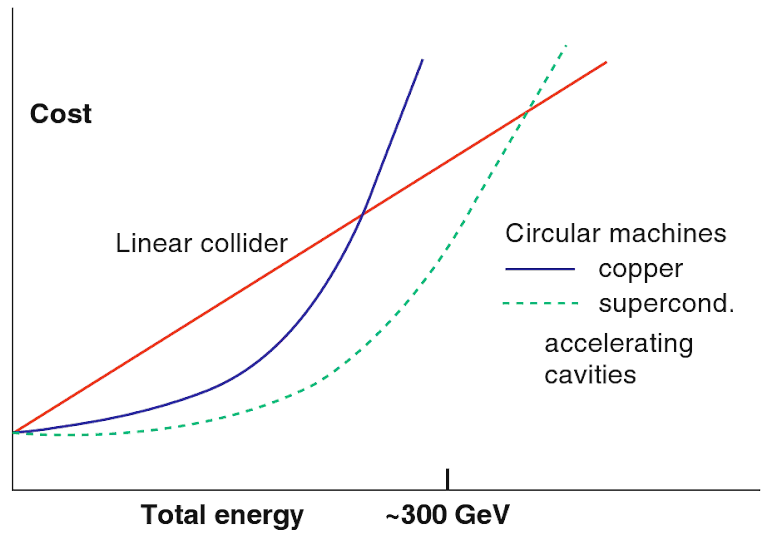
\includegraphics[width=0.55\textwidth]{Figures/Collider_costs.png}
\caption[Construction cost of linear and circular colliders]{Relations between the construction cost and the center-of-mass energy for linear and circular \positron\electron colliders~\cite[p. 13]{Schopper}.}
\label{fig:Costs}
\end{figure}